
\begin{figure}
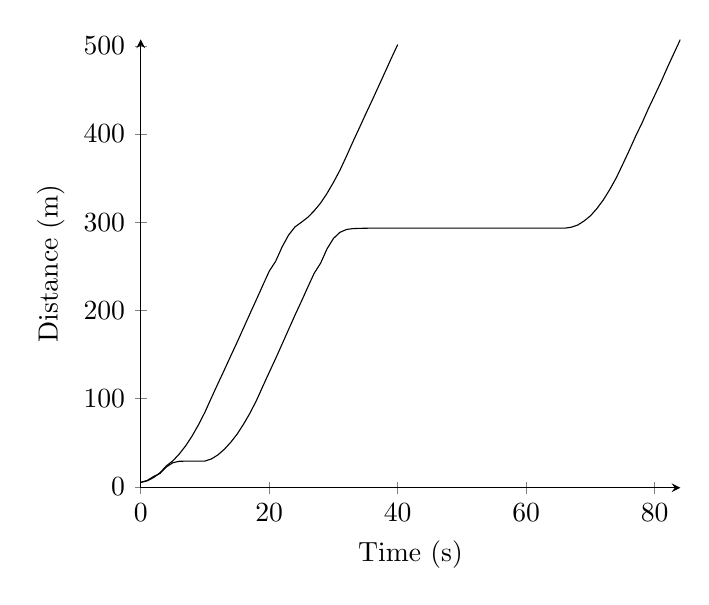
\begin{tikzpicture}
\begin{axis}[
legend style={anchor=west},
axis x line=bottom,
axis y line=left,
ymin=-1,
xlabel=Time (s),
ylabel=Distance (m),
]
\addplot[] coordinates {
(0, 5.1)
(1, 6.83048050696)
(2, 10.5731880958)
(3, 16.0313307799)
(4, 23.9111939491)
(5, 29.5550996829)
(6, 37.342390298)
(7, 46.6484631223)
(8, 57.7656222519)
(9, 70.5765570039)
(10, 84.847632322)
(11, 101.051813443)
(12, 116.898510643)
(13, 132.452928301)
(14, 148.308743307)
(15, 164.006689237)
(16, 180.158985418)
(17, 196.358728666)
(18, 212.31444653)
(19, 228.513184813)
(20, 244.563184512)
(21, 255.792602076)
(22, 271.980357729)
(23, 285.324699256)
(24, 294.677576396)
(25, 299.973726927)
(26, 305.569190399)
(27, 313.016428614)
(28, 321.806371819)
(29, 332.830350051)
(30, 345.234625559)
(31, 358.924842238)
(32, 374.54598921)
(33, 390.860206218)
(34, 406.518850071)
(35, 422.422779725)
(36, 437.936676205)
(37, 453.809404349)
(38, 469.798420223)
(39, 485.880152786)
(40, 501.388793656)
};
\addplot[] coordinates {
(0, 5.1)
(1, 7.25817123884)
(2, 11.7621658331)
(3, 15.2288149051)
(4, 22.7103906676)
(5, 27.3928158903)
(6, 29.0219514679)
(7, 29.1761366441)
(8, 29.2501106184)
(9, 29.262426998)
(10, 29.262426998)
(11, 31.6709933085)
(12, 36.2065682294)
(13, 42.5698740141)
(14, 50.4832293979)
(15, 59.8077028589)
(16, 71.0627584294)
(17, 83.620318873)
(18, 97.7786755746)
(19, 113.998657524)
(20, 129.899529075)
(21, 145.569739128)
(22, 161.852825501)
(23, 178.252426746)
(24, 194.568153631)
(25, 210.244953332)
(26, 226.390065802)
(27, 242.22812742)
(28, 253.671782853)
(29, 269.879760106)
(30, 281.653825309)
(31, 288.527243985)
(32, 291.736365826)
(33, 292.770056469)
(34, 293.031775862)
(35, 293.236593899)
(36, 293.263361068)
(37, 293.263361068)
(38, 293.263361068)
(39, 293.263361068)
(40, 293.263361068)
(41, 293.263361068)
(42, 293.263361068)
(43, 293.263361068)
(44, 293.263361068)
(45, 293.263361068)
(46, 293.263361068)
(47, 293.263361068)
(48, 293.263361068)
(49, 293.263361068)
(50, 293.263361068)
(51, 293.263361068)
(52, 293.263361068)
(53, 293.263361068)
(54, 293.263361068)
(55, 293.263361068)
(56, 293.263361068)
(57, 293.263361068)
(58, 293.263361068)
(59, 293.263361068)
(60, 293.263361068)
(61, 293.263361068)
(62, 293.263361068)
(63, 293.263361068)
(64, 293.263361068)
(65, 293.263361068)
(66, 293.263361068)
(67, 294.299384631)
(68, 296.742932418)
(69, 301.380904622)
(70, 307.269654837)
(71, 315.464555146)
(72, 325.266411639)
(73, 336.992874068)
(74, 350.045224857)
(75, 365.272419345)
(76, 380.800245668)
(77, 397.036773209)
(78, 412.065381441)
(79, 428.480467817)
(80, 443.814241524)
(81, 459.322303191)
(82, 475.797328112)
(83, 491.612548679)
(84, 507.213634475)
};

\end{axis}
\end{tikzpicture}
\label{tik:0:6_O, 6_O.-30, 5_N, 4_N, 4_N.-60, 2_V}
\caption{0 percent diving with GSC on route $6_O, 6_O.-30, 5_N, 4_N, 4_N.-60, 2_V$}
\end{figure}
